\documentclass[11pt]{article}
\usepackage[textwidth=18.0cm, textheight=23.0cm, top=2.0cm]{geometry}
\usepackage{pst-all}
\usepackage{amssymb}
\usepackage{tikz}
\usepackage{underscore}\begin{document}
\pagestyle{empty}


ClassName: \underline{\textbf{Class_09.2bp-4}}
\par
BinSize: \underline{\textbf{100 × 100}}
\par
ReduceSize: \underline{\textbf{99 × 100}}
\par
TypeNum: \underline{\textbf{20}}
\par
Num: \underline{\textbf{20}}
\par
OutS: \underline{\textbf{160000}}
\par
InS: \underline{\textbf{98570}}
\par
Rate: \underline{\textbf{0.616}}
\par
UB: \underline{\textbf{16}}
\par
LB0: \underline{\textbf{16}}
\par
LB: \underline{\textbf{16}}
\par
LBWithCut: \underline{\textbf{16}}
\par
NodeCut: \underline{\textbf{0}}
\par
ExtendedNodeCnt: \underline{\textbf{1}}
\par
GenNodeCnt: \underline{\textbf{1}}
\par
PrimalNode: \underline{\textbf{0}}
\par
ColumnCount: \underline{\textbf{16}}
\par
TotalCutCount: \underline{\textbf{0}}
\par
RootCutCount: \underline{\textbf{0}}
\par
LPSolverCnt: \underline{\textbf{1}}
\par
PricingSolverCnt: \underline{\textbf{0}}
\par
BranchAndBoundNum: \underline{\textbf{1}}
\par
isOpt: \underline{\textbf{true}}
\par
TimeOnInitSolution: \underline{\textbf{600.000 s}}
\par
TimeOnPrimal: \underline{\textbf{0.000 s}}
\par
TimeOnPricing: \underline{\textbf{0.000 s}}
\par
TimeOnRmp: \underline{\textbf{0.062 s}}
\par
TotalTime: \underline{\textbf{600.313 s}}
\par
\newpage


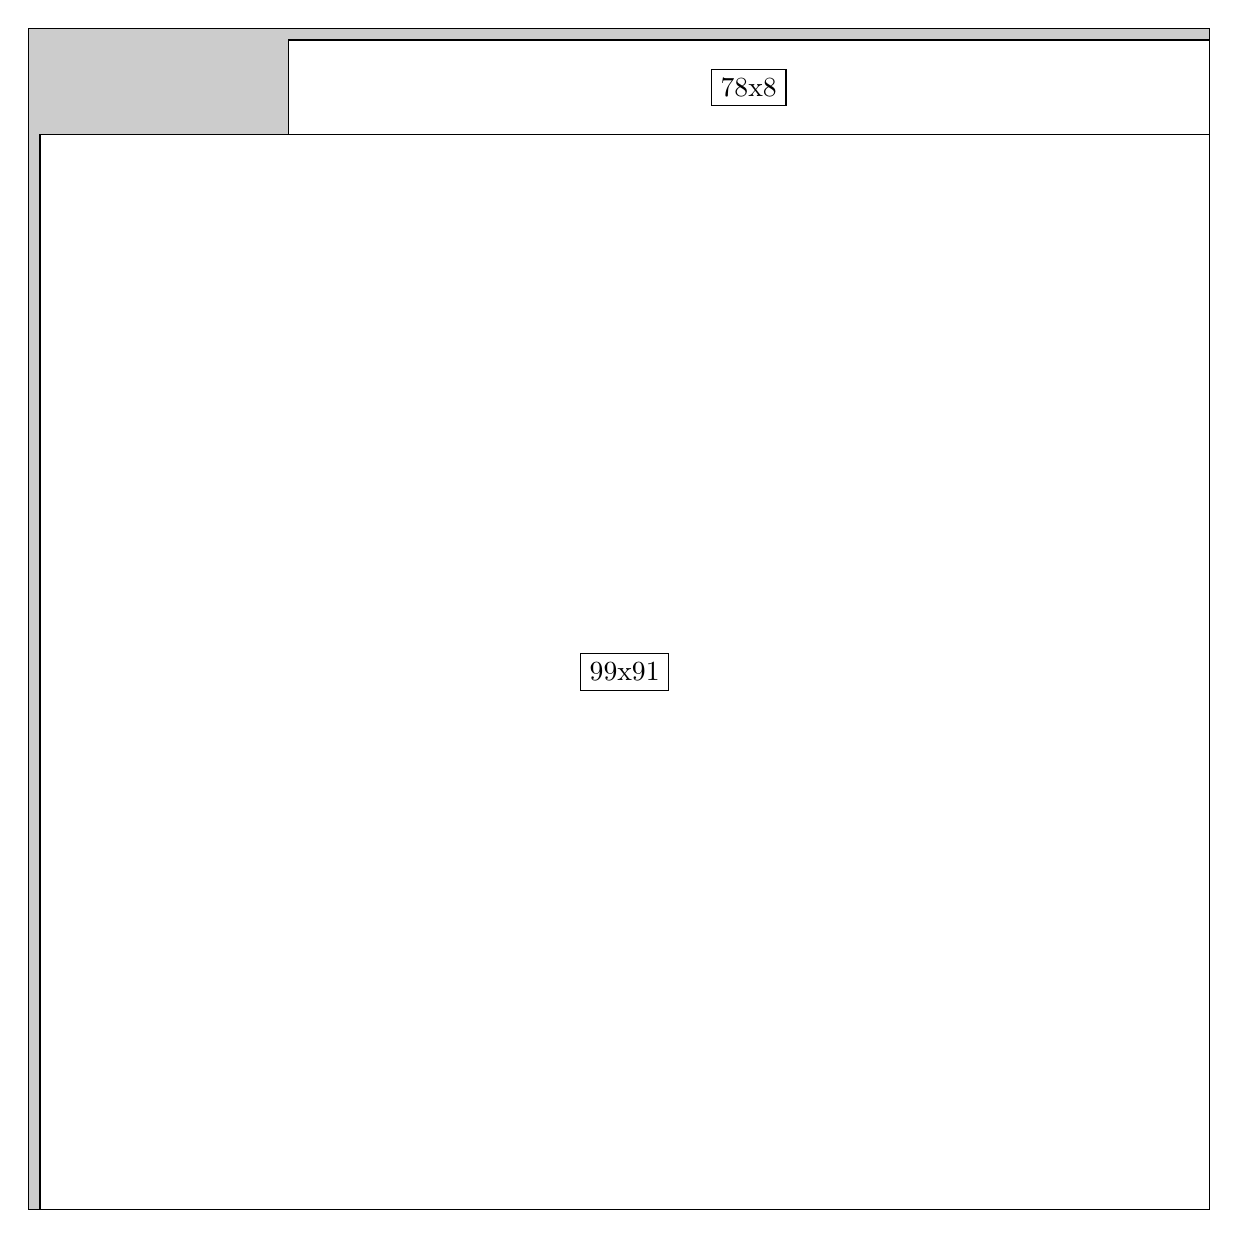
\begin{tikzpicture}[shorten >=1pt,scale=1.0,every node/.style={scale=1.0},->]
\tikzstyle{vertex}=[circle,fill=black!25,minimum size=14pt,inner sep=0pt]
\filldraw[fill=gray!40!white, draw=black] (0,0) rectangle (15.0,15.0);
\foreach \name/\x/\y/\w/\h in {99x91/0.15/0.0/14.85/13.65,78x8/3.3/13.65/11.7/1.2}
\filldraw[fill=white!40!white, draw=black] (\x,\y) rectangle node[draw] (\name) {\name} ++(\w,\h);
\end{tikzpicture}


w =99 , h =91 , x =1 , y =0 , v =9009
\par
w =78 , h =8 , x =22 , y =91 , v =624
\par
\newpage


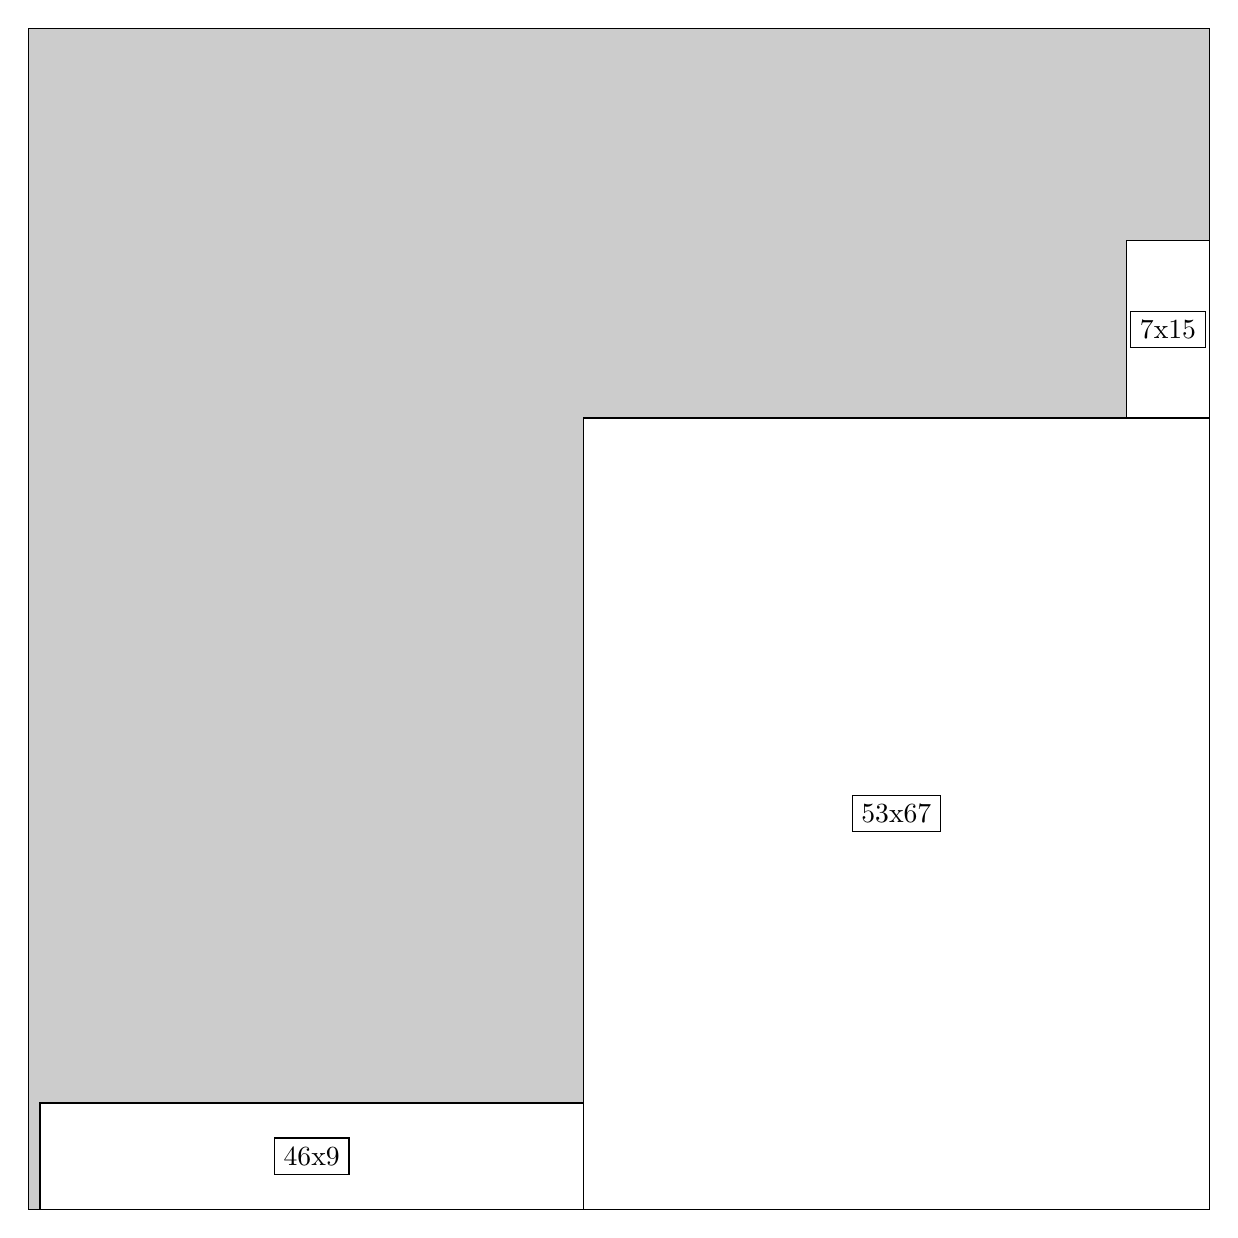
\begin{tikzpicture}[shorten >=1pt,scale=1.0,every node/.style={scale=1.0},->]
\tikzstyle{vertex}=[circle,fill=black!25,minimum size=14pt,inner sep=0pt]
\filldraw[fill=gray!40!white, draw=black] (0,0) rectangle (15.0,15.0);
\foreach \name/\x/\y/\w/\h in {53x67/7.05/0.0/7.949999999999999/10.049999999999999,46x9/0.15/0.0/6.8999999999999995/1.3499999999999999,7x15/13.95/10.049999999999999/1.05/2.25}
\filldraw[fill=white!40!white, draw=black] (\x,\y) rectangle node[draw] (\name) {\name} ++(\w,\h);
\end{tikzpicture}


w =53 , h =67 , x =47 , y =0 , v =3551
\par
w =46 , h =9 , x =1 , y =0 , v =414
\par
w =7 , h =15 , x =93 , y =67 , v =105
\par
\newpage


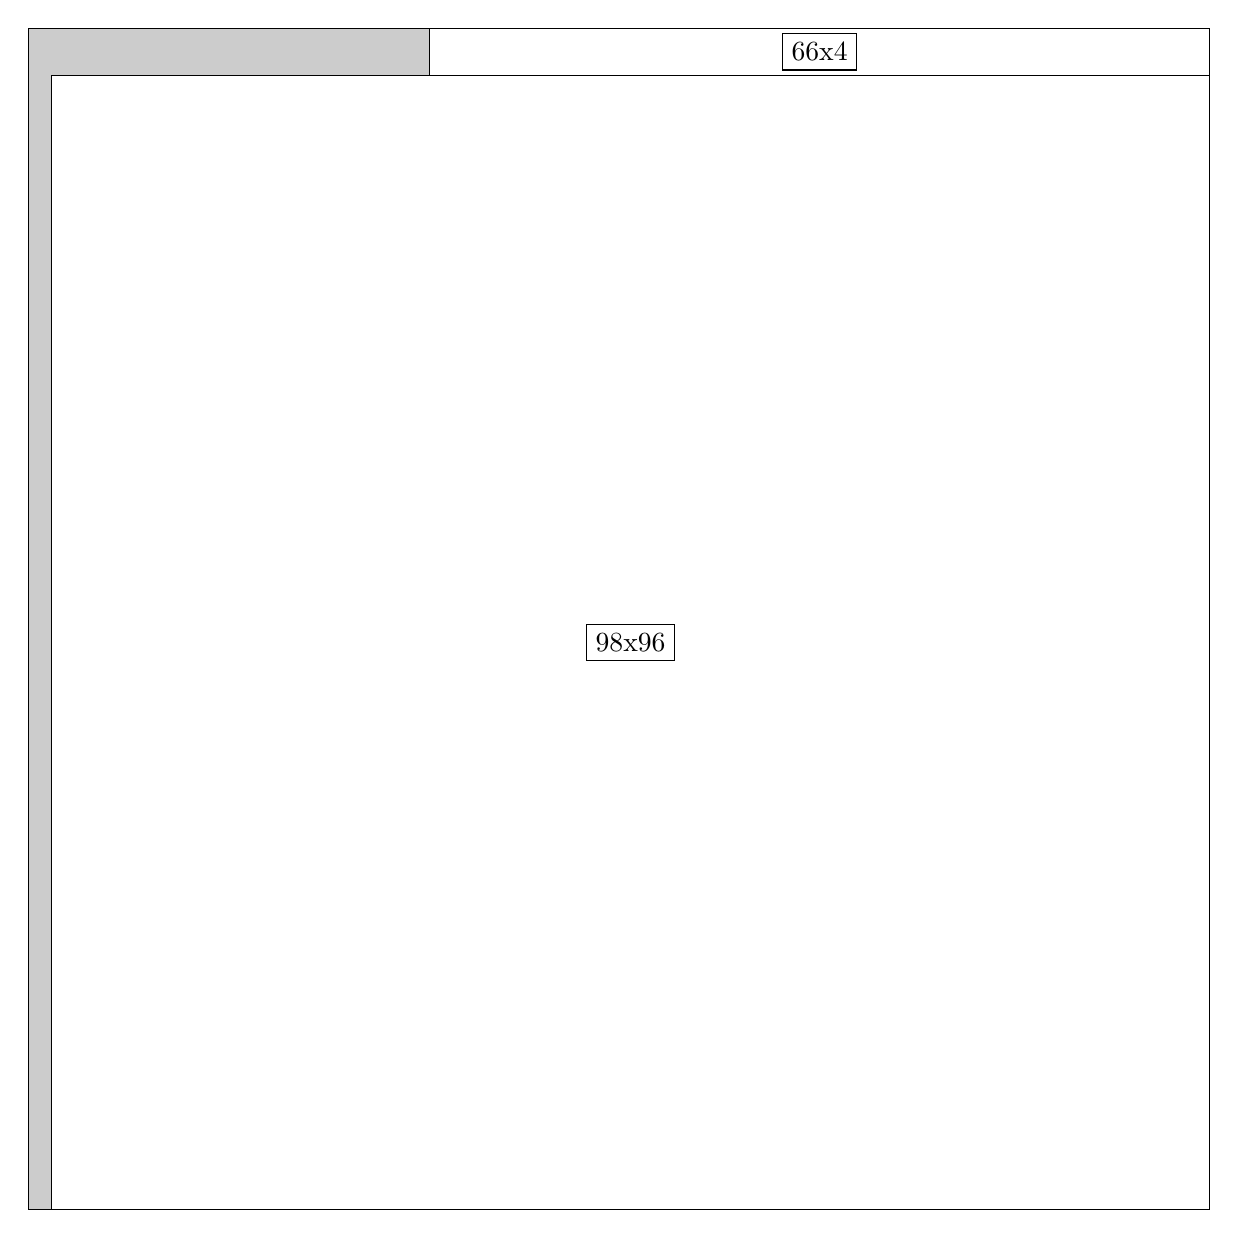
\begin{tikzpicture}[shorten >=1pt,scale=1.0,every node/.style={scale=1.0},->]
\tikzstyle{vertex}=[circle,fill=black!25,minimum size=14pt,inner sep=0pt]
\filldraw[fill=gray!40!white, draw=black] (0,0) rectangle (15.0,15.0);
\foreach \name/\x/\y/\w/\h in {98x96/0.3/0.0/14.7/14.399999999999999,66x4/5.1/14.399999999999999/9.9/0.6}
\filldraw[fill=white!40!white, draw=black] (\x,\y) rectangle node[draw] (\name) {\name} ++(\w,\h);
\end{tikzpicture}


w =98 , h =96 , x =2 , y =0 , v =9408
\par
w =66 , h =4 , x =34 , y =96 , v =264
\par
\newpage


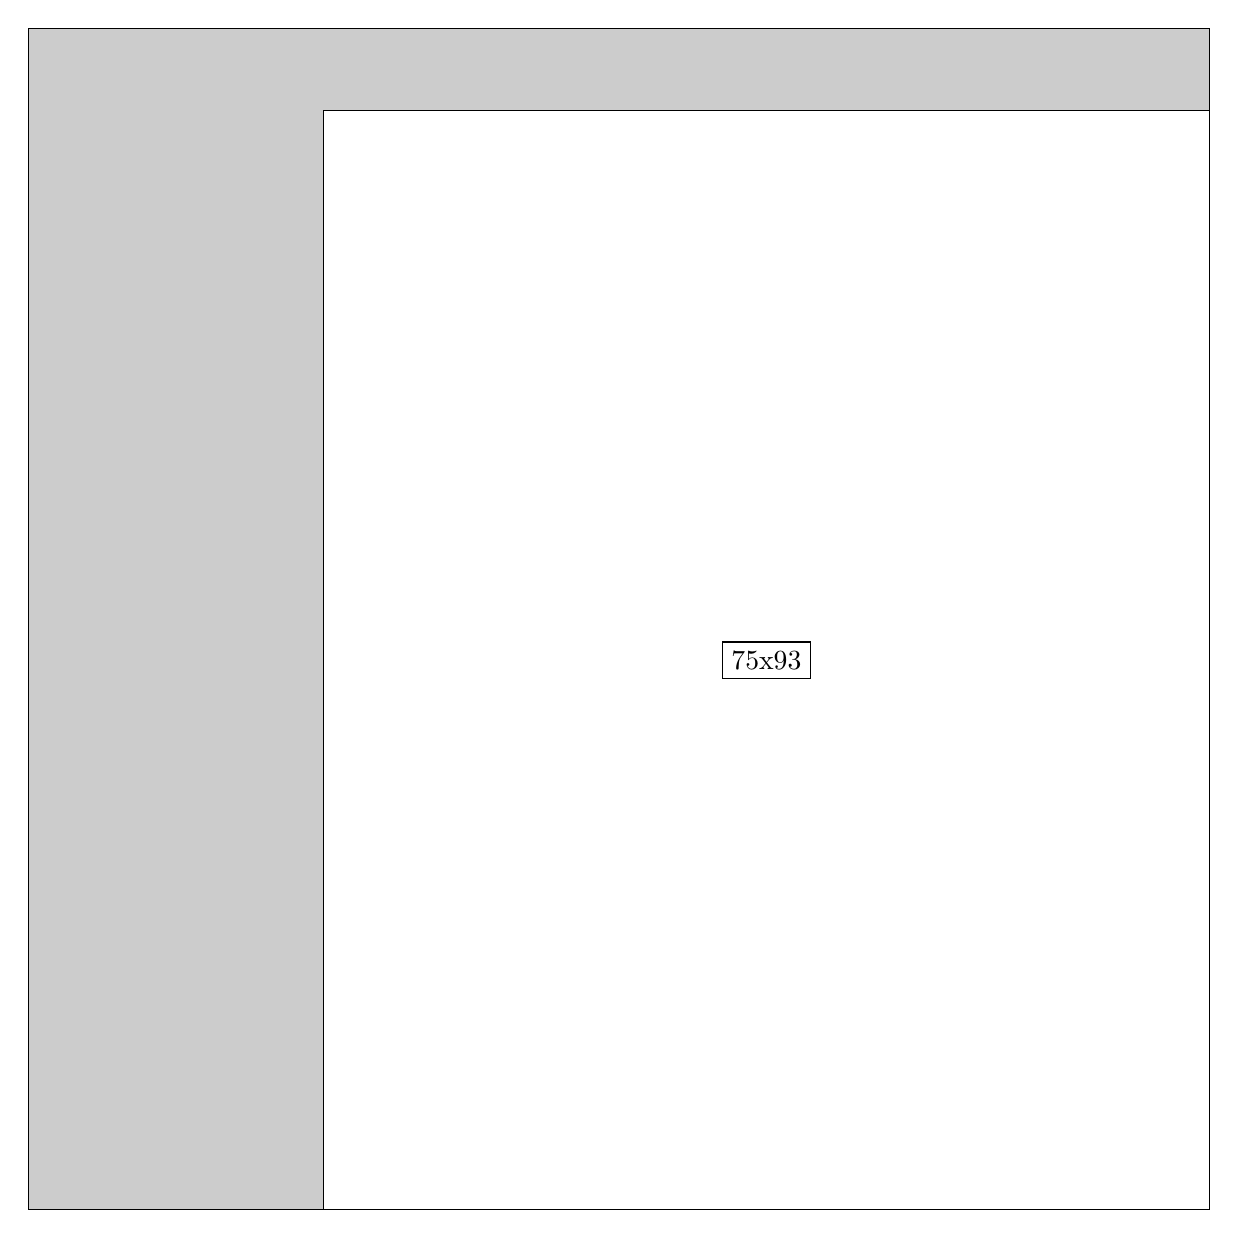
\begin{tikzpicture}[shorten >=1pt,scale=1.0,every node/.style={scale=1.0},->]
\tikzstyle{vertex}=[circle,fill=black!25,minimum size=14pt,inner sep=0pt]
\filldraw[fill=gray!40!white, draw=black] (0,0) rectangle (15.0,15.0);
\foreach \name/\x/\y/\w/\h in {75x93/3.75/0.0/11.25/13.95}
\filldraw[fill=white!40!white, draw=black] (\x,\y) rectangle node[draw] (\name) {\name} ++(\w,\h);
\end{tikzpicture}


w =75 , h =93 , x =25 , y =0 , v =6975
\par
\newpage



\begin{tikzpicture}[shorten >=1pt,scale=1.0,every node/.style={scale=1.0},->]
\tikzstyle{vertex}=[circle,fill=black!25,minimum size=14pt,inner sep=0pt]
\filldraw[fill=gray!40!white, draw=black] (0,0) rectangle (15.0,15.0);
\foreach \name/\x/\y/\w/\h in {69x98/4.6499999999999995/0.0/10.35/14.7}
\filldraw[fill=white!40!white, draw=black] (\x,\y) rectangle node[draw] (\name) {\name} ++(\w,\h);
\end{tikzpicture}


w =69 , h =98 , x =31 , y =0 , v =6762
\par
\newpage


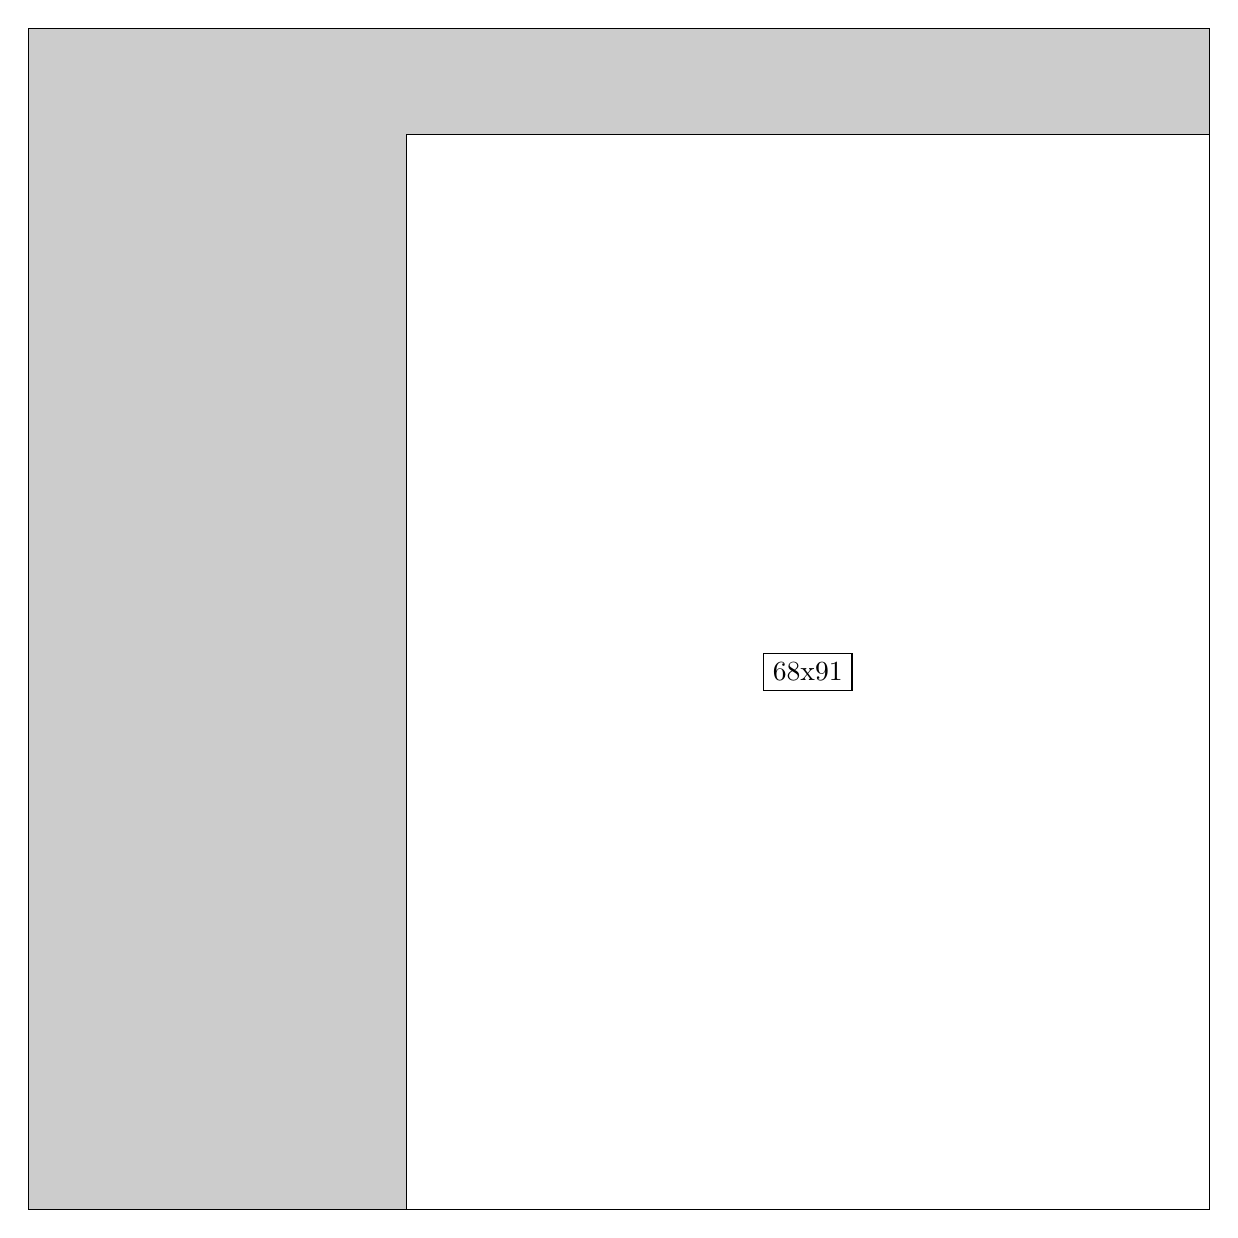
\begin{tikzpicture}[shorten >=1pt,scale=1.0,every node/.style={scale=1.0},->]
\tikzstyle{vertex}=[circle,fill=black!25,minimum size=14pt,inner sep=0pt]
\filldraw[fill=gray!40!white, draw=black] (0,0) rectangle (15.0,15.0);
\foreach \name/\x/\y/\w/\h in {68x91/4.8/0.0/10.2/13.65}
\filldraw[fill=white!40!white, draw=black] (\x,\y) rectangle node[draw] (\name) {\name} ++(\w,\h);
\end{tikzpicture}


w =68 , h =91 , x =32 , y =0 , v =6188
\par
\newpage


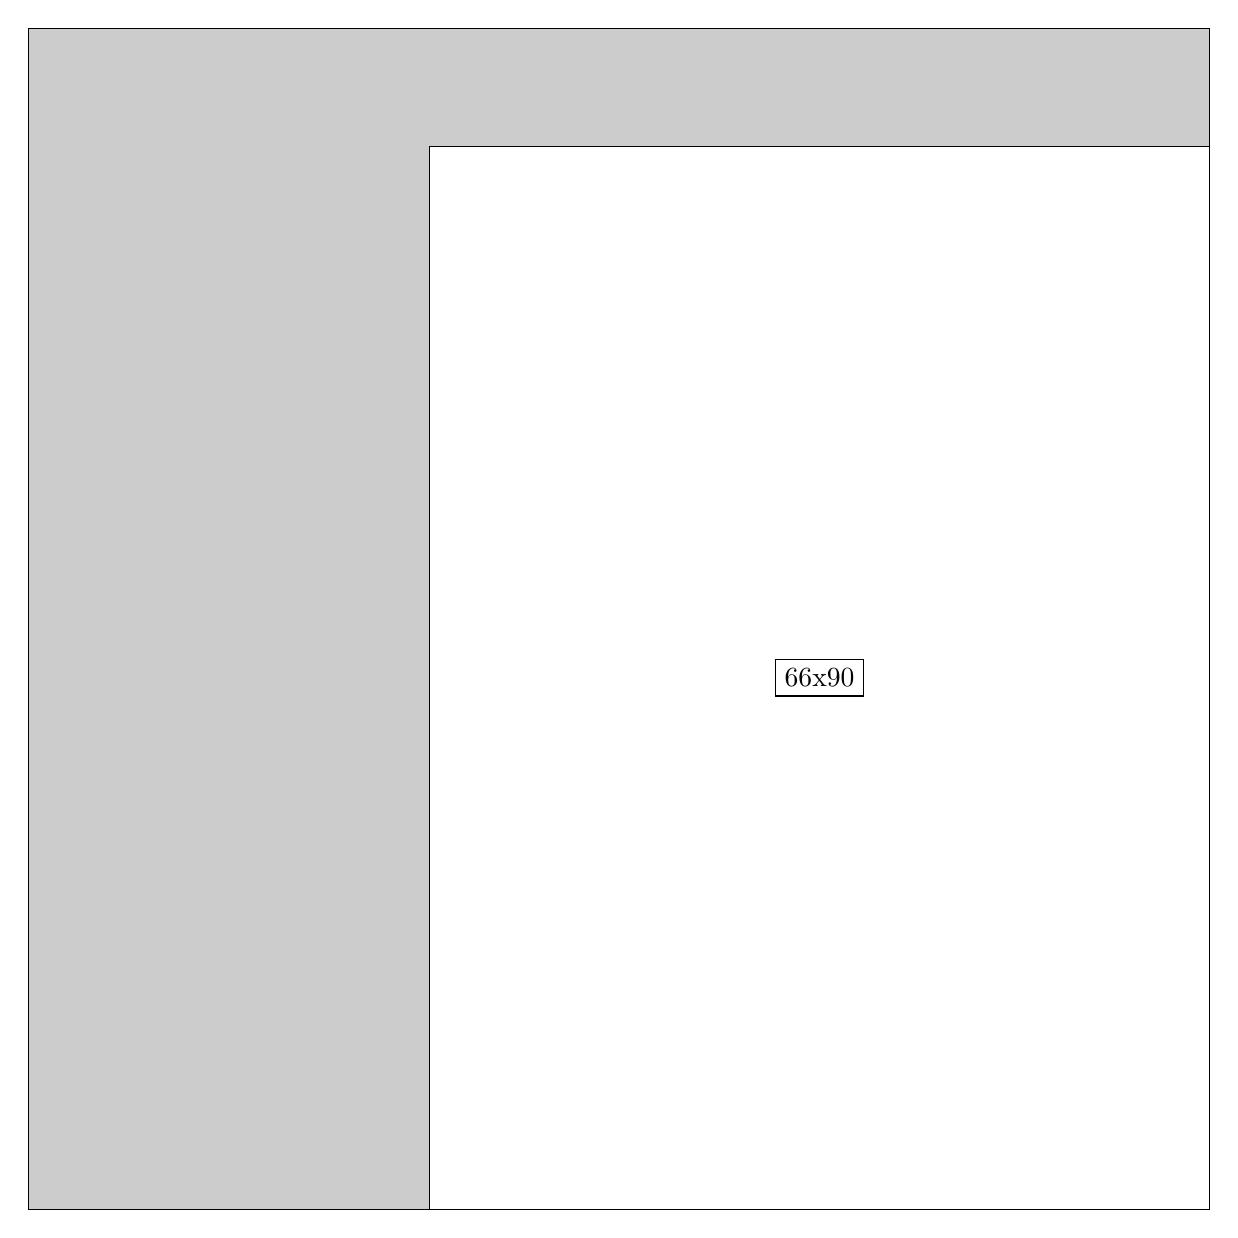
\begin{tikzpicture}[shorten >=1pt,scale=1.0,every node/.style={scale=1.0},->]
\tikzstyle{vertex}=[circle,fill=black!25,minimum size=14pt,inner sep=0pt]
\filldraw[fill=gray!40!white, draw=black] (0,0) rectangle (15.0,15.0);
\foreach \name/\x/\y/\w/\h in {66x90/5.1/0.0/9.9/13.5}
\filldraw[fill=white!40!white, draw=black] (\x,\y) rectangle node[draw] (\name) {\name} ++(\w,\h);
\end{tikzpicture}


w =66 , h =90 , x =34 , y =0 , v =5940
\par
\newpage


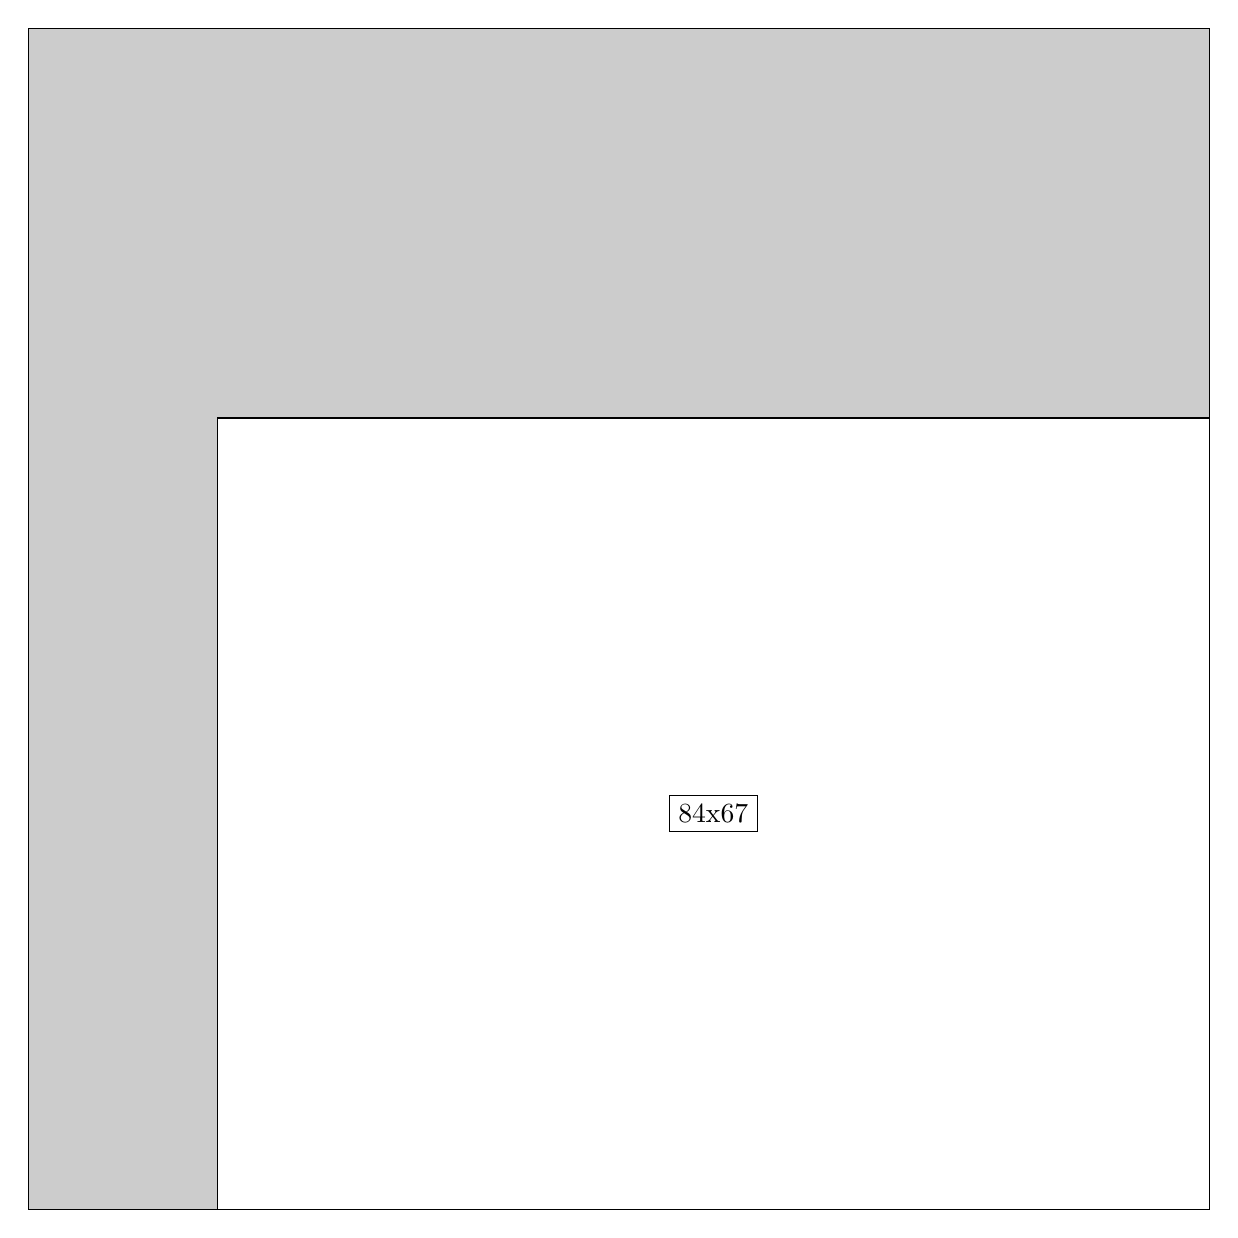
\begin{tikzpicture}[shorten >=1pt,scale=1.0,every node/.style={scale=1.0},->]
\tikzstyle{vertex}=[circle,fill=black!25,minimum size=14pt,inner sep=0pt]
\filldraw[fill=gray!40!white, draw=black] (0,0) rectangle (15.0,15.0);
\foreach \name/\x/\y/\w/\h in {84x67/2.4/0.0/12.6/10.049999999999999}
\filldraw[fill=white!40!white, draw=black] (\x,\y) rectangle node[draw] (\name) {\name} ++(\w,\h);
\end{tikzpicture}


w =84 , h =67 , x =16 , y =0 , v =5628
\par
\newpage



\begin{tikzpicture}[shorten >=1pt,scale=1.0,every node/.style={scale=1.0},->]
\tikzstyle{vertex}=[circle,fill=black!25,minimum size=14pt,inner sep=0pt]
\filldraw[fill=gray!40!white, draw=black] (0,0) rectangle (15.0,15.0);
\foreach \name/\x/\y/\w/\h in {96x76/0.6/0.0/14.399999999999999/11.4}
\filldraw[fill=white!40!white, draw=black] (\x,\y) rectangle node[draw] (\name) {\name} ++(\w,\h);
\end{tikzpicture}


w =96 , h =76 , x =4 , y =0 , v =7296
\par
\newpage


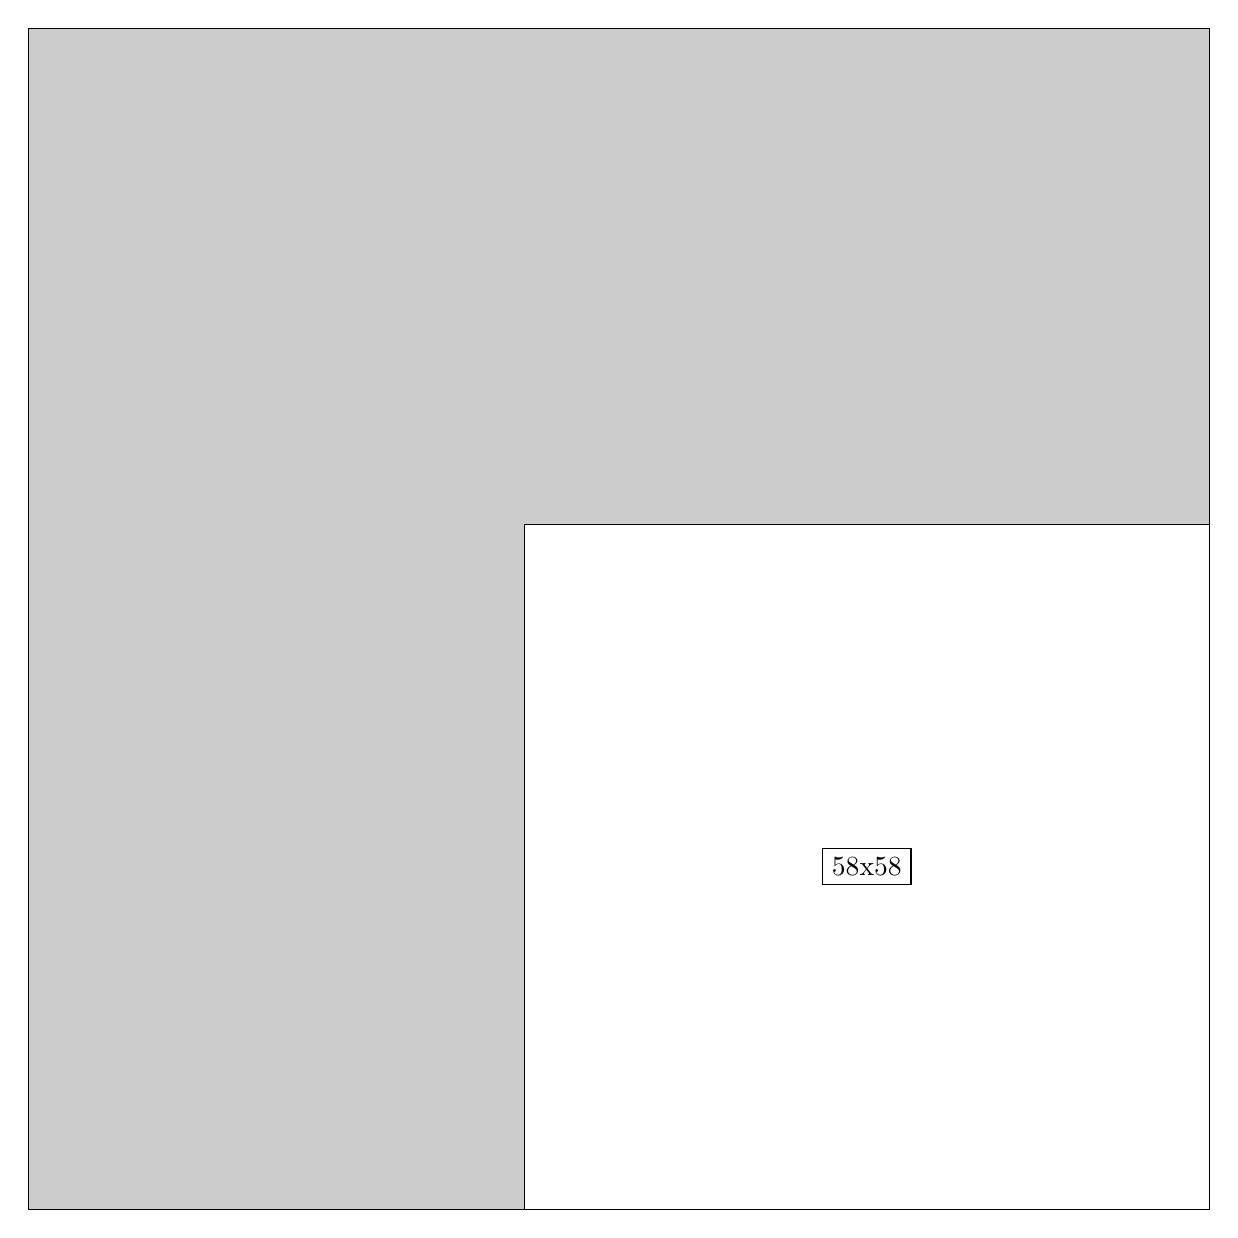
\begin{tikzpicture}[shorten >=1pt,scale=1.0,every node/.style={scale=1.0},->]
\tikzstyle{vertex}=[circle,fill=black!25,minimum size=14pt,inner sep=0pt]
\filldraw[fill=gray!40!white, draw=black] (0,0) rectangle (15.0,15.0);
\foreach \name/\x/\y/\w/\h in {58x58/6.3/0.0/8.7/8.7}
\filldraw[fill=white!40!white, draw=black] (\x,\y) rectangle node[draw] (\name) {\name} ++(\w,\h);
\end{tikzpicture}


w =58 , h =58 , x =42 , y =0 , v =3364
\par
\newpage


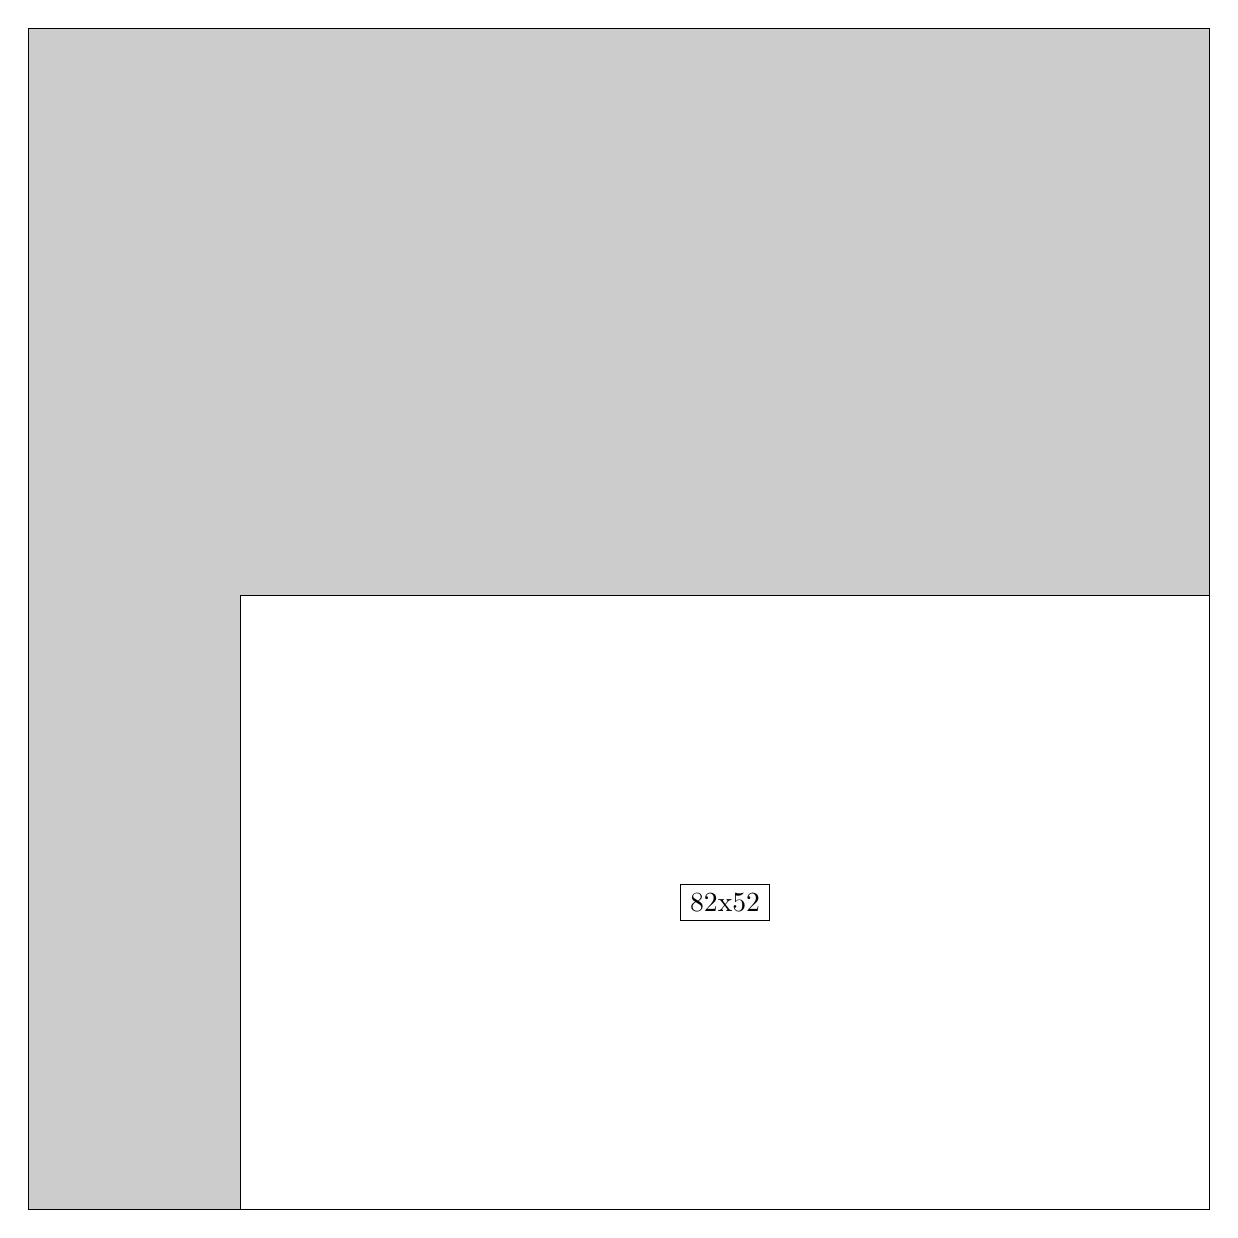
\begin{tikzpicture}[shorten >=1pt,scale=1.0,every node/.style={scale=1.0},->]
\tikzstyle{vertex}=[circle,fill=black!25,minimum size=14pt,inner sep=0pt]
\filldraw[fill=gray!40!white, draw=black] (0,0) rectangle (15.0,15.0);
\foreach \name/\x/\y/\w/\h in {82x52/2.6999999999999997/0.0/12.299999999999999/7.8}
\filldraw[fill=white!40!white, draw=black] (\x,\y) rectangle node[draw] (\name) {\name} ++(\w,\h);
\end{tikzpicture}


w =82 , h =52 , x =18 , y =0 , v =4264
\par
\newpage


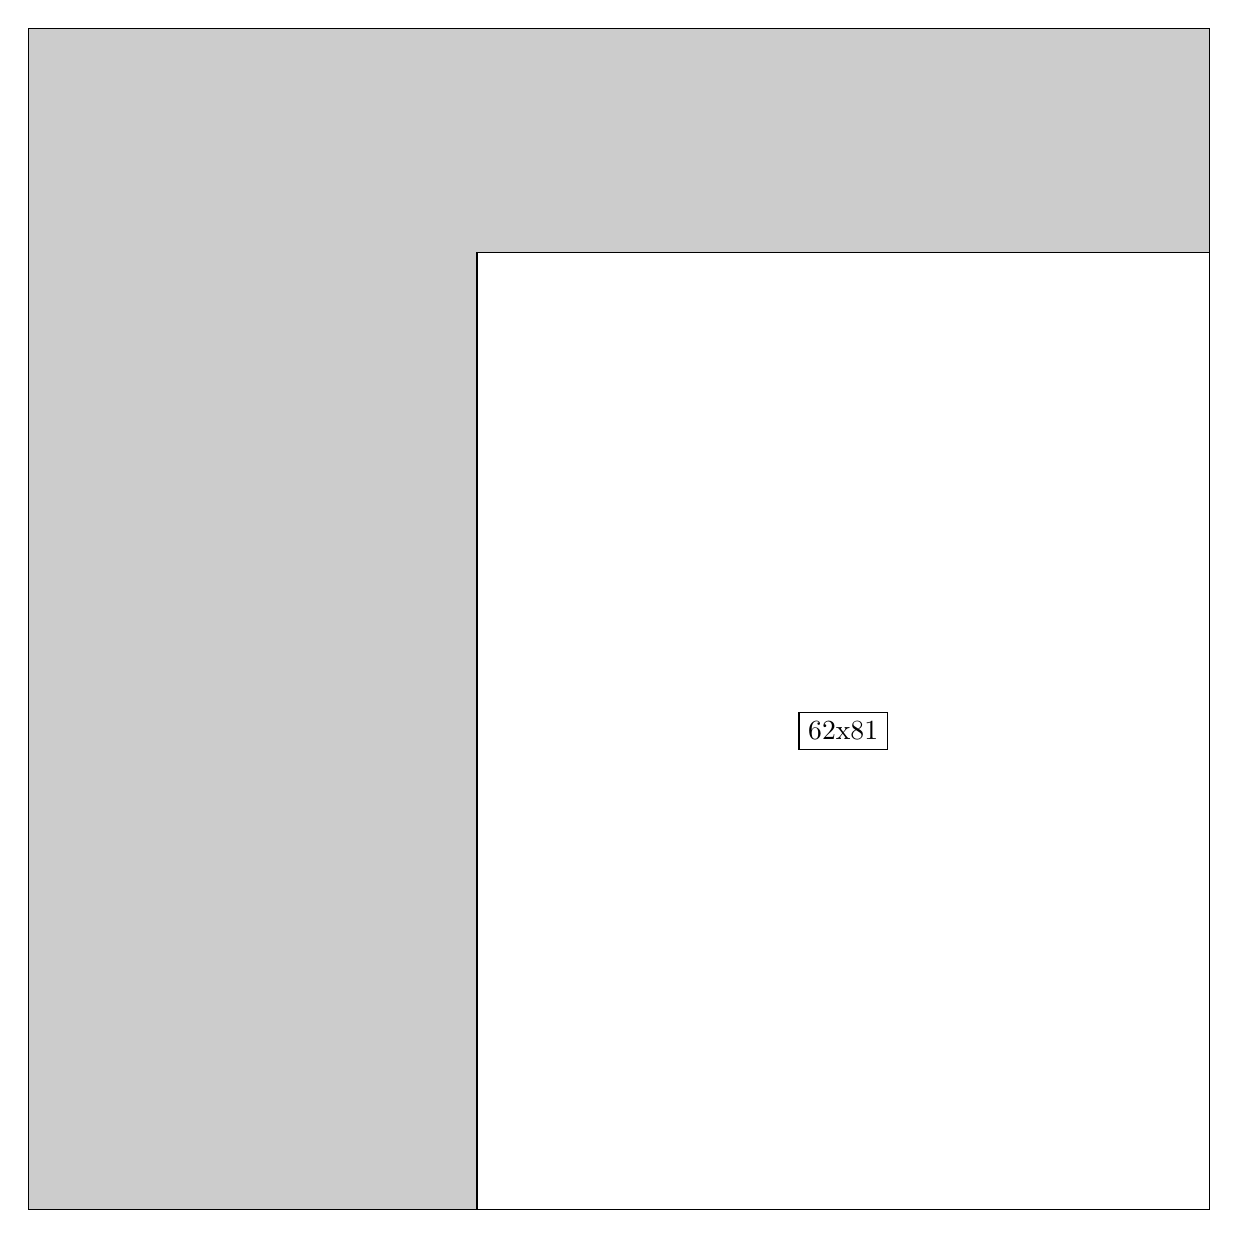
\begin{tikzpicture}[shorten >=1pt,scale=1.0,every node/.style={scale=1.0},->]
\tikzstyle{vertex}=[circle,fill=black!25,minimum size=14pt,inner sep=0pt]
\filldraw[fill=gray!40!white, draw=black] (0,0) rectangle (15.0,15.0);
\foreach \name/\x/\y/\w/\h in {62x81/5.7/0.0/9.299999999999999/12.15}
\filldraw[fill=white!40!white, draw=black] (\x,\y) rectangle node[draw] (\name) {\name} ++(\w,\h);
\end{tikzpicture}


w =62 , h =81 , x =38 , y =0 , v =5022
\par
\newpage



\begin{tikzpicture}[shorten >=1pt,scale=1.0,every node/.style={scale=1.0},->]
\tikzstyle{vertex}=[circle,fill=black!25,minimum size=14pt,inner sep=0pt]
\filldraw[fill=gray!40!white, draw=black] (0,0) rectangle (15.0,15.0);
\foreach \name/\x/\y/\w/\h in {95x55/0.75/0.0/14.25/8.25}
\filldraw[fill=white!40!white, draw=black] (\x,\y) rectangle node[draw] (\name) {\name} ++(\w,\h);
\end{tikzpicture}


w =95 , h =55 , x =5 , y =0 , v =5225
\par
\newpage


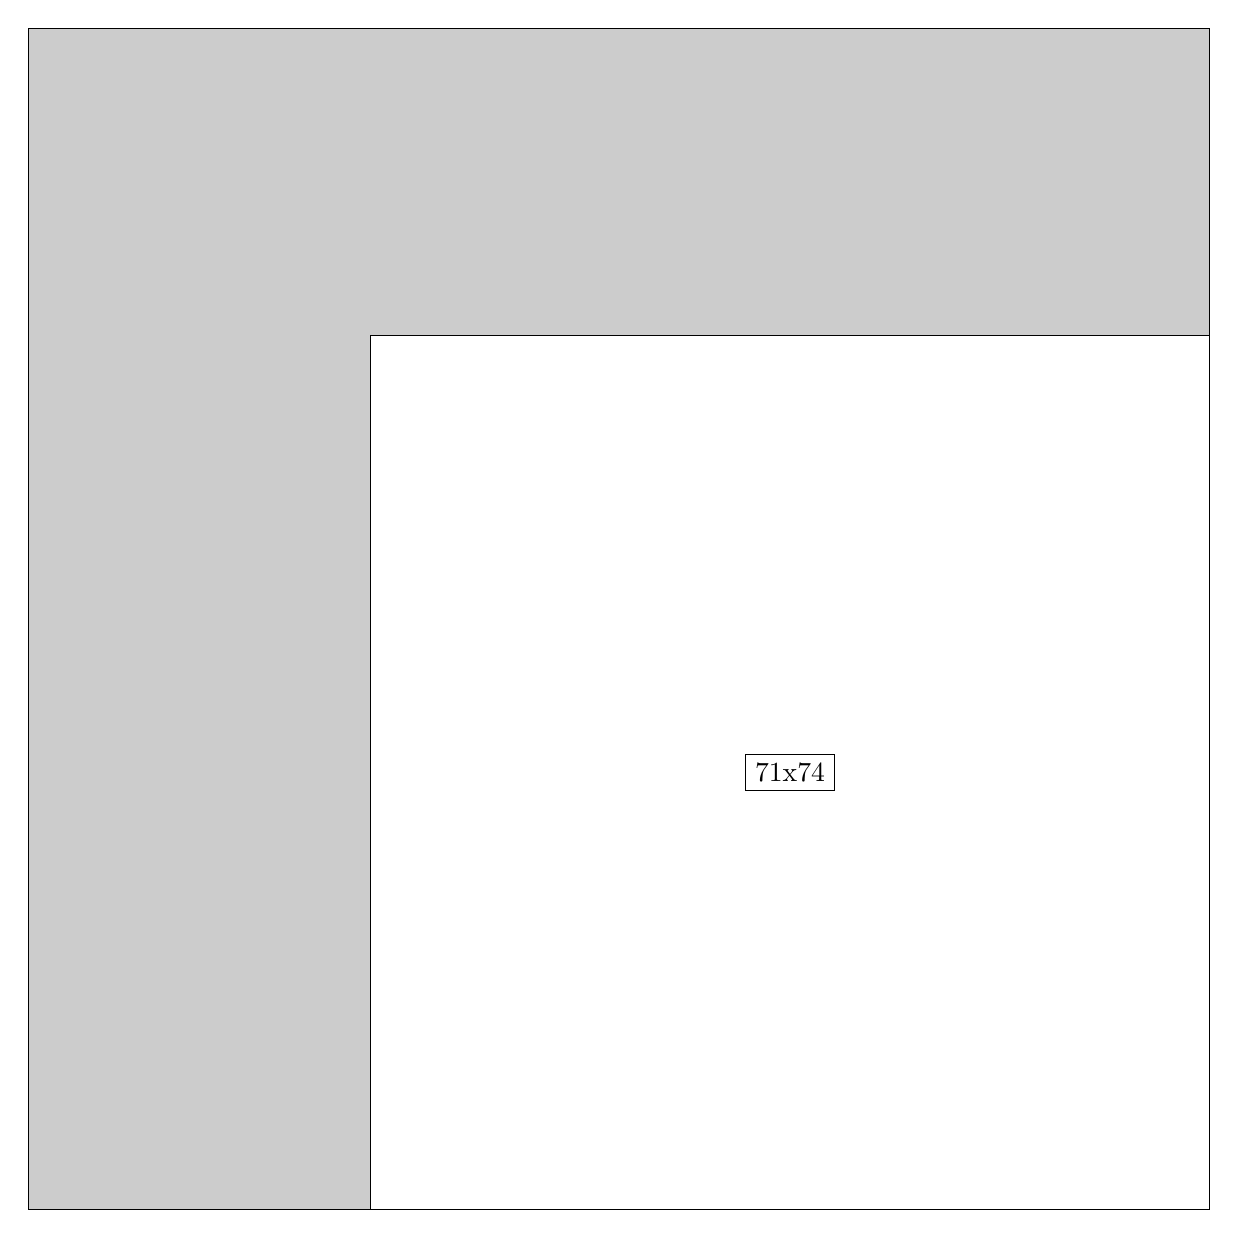
\begin{tikzpicture}[shorten >=1pt,scale=1.0,every node/.style={scale=1.0},->]
\tikzstyle{vertex}=[circle,fill=black!25,minimum size=14pt,inner sep=0pt]
\filldraw[fill=gray!40!white, draw=black] (0,0) rectangle (15.0,15.0);
\foreach \name/\x/\y/\w/\h in {71x74/4.35/0.0/10.65/11.1}
\filldraw[fill=white!40!white, draw=black] (\x,\y) rectangle node[draw] (\name) {\name} ++(\w,\h);
\end{tikzpicture}


w =71 , h =74 , x =29 , y =0 , v =5254
\par
\newpage



\begin{tikzpicture}[shorten >=1pt,scale=1.0,every node/.style={scale=1.0},->]
\tikzstyle{vertex}=[circle,fill=black!25,minimum size=14pt,inner sep=0pt]
\filldraw[fill=gray!40!white, draw=black] (0,0) rectangle (15.0,15.0);
\foreach \name/\x/\y/\w/\h in {99x61/0.15/0.0/14.85/9.15}
\filldraw[fill=white!40!white, draw=black] (\x,\y) rectangle node[draw] (\name) {\name} ++(\w,\h);
\end{tikzpicture}


w =99 , h =61 , x =1 , y =0 , v =6039
\par
\newpage


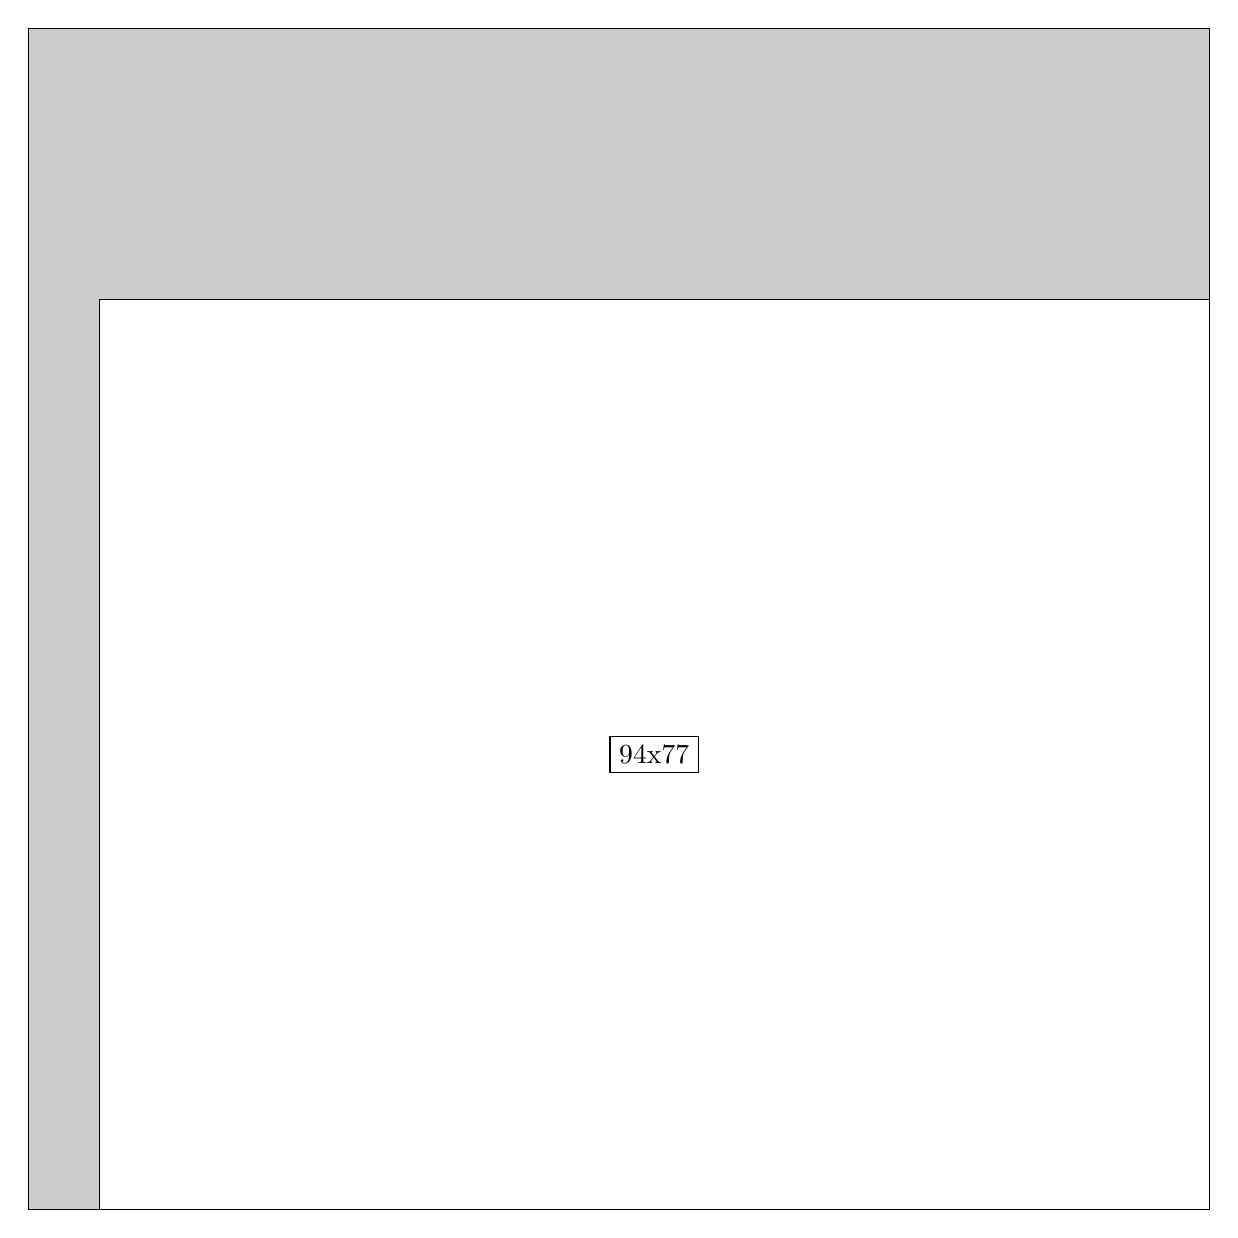
\begin{tikzpicture}[shorten >=1pt,scale=1.0,every node/.style={scale=1.0},->]
\tikzstyle{vertex}=[circle,fill=black!25,minimum size=14pt,inner sep=0pt]
\filldraw[fill=gray!40!white, draw=black] (0,0) rectangle (15.0,15.0);
\foreach \name/\x/\y/\w/\h in {94x77/0.8999999999999999/0.0/14.1/11.549999999999999}
\filldraw[fill=white!40!white, draw=black] (\x,\y) rectangle node[draw] (\name) {\name} ++(\w,\h);
\end{tikzpicture}


w =94 , h =77 , x =6 , y =0 , v =7238
\par
\newpage


\end{document}